\documentclass[a4paper]{article}
\usepackage[T1]{fontenc}
\usepackage[utf8]{inputenc}

\usepackage{fancyhdr} 
% \usepackage[]{cite}
\usepackage[backend=biber,style=ieee,maxcitenames=2,mincitenames=1]{biblatex}
\usepackage{lastpage} 
\usepackage{extramarks} 
\usepackage{graphicx,color}
\usepackage{anysize}
\usepackage{amsmath}
% \usepackage{natbib}
\usepackage{caption}
\usepackage{float}
\usepackage{url}
\usepackage{listings}
\usepackage[svgnames]{xcolor}
\usepackage[colorlinks=true, allcolors=black]{hyperref}
\usepackage[small]{titlesec}
\usepackage[version=4]{mhchem}
\usepackage{linegoal}
\usepackage{subcaption}
\usepackage{media9}
\usepackage{tcolorbox}
\usepackage{lmodern}


\textwidth=6.5in
\linespread{1.0} % Line spacing
\renewcommand{\familydefault}{\sfdefault}

% \titleformat{\section}
% {\normalfont\bfseries}
% {\thesection.}{0.75em}{}

\titlespacing{\section}{0pt}{10pt}{5pt}

%% includescalefigure:
%% \includescalefigure{label}{short caption}{long caption}{scale}{filename}
%% - includes a figure with a given label, a short caption for the table of contents and a longer caption that describes the figure in some detail and a scale factor 'scale'
\newcommand{\includescalefigure}[5]{
\begin{figure}[!ht]
\centering
\includegraphics[width=#4\linewidth]{#5}
\captionsetup{width=.8\linewidth} 
\caption[#2]{#3}
\label{#1}
\end{figure}
}

\newcommand{\imageinners}[4]{
\begin{subfigure}{0.4\linewidth}
\includegraphics[width=\linewidth]{#4}
\captionsetup{width=.8\linewidth} 
\caption[#2]{#3}
\label{#1}
\end{subfigure}
}

%% includefigure:
%% \includefigure{label}{short caption}{long caption}{filename}
%% - includes a figure with a given label, a short caption for the table of contents and a longer caption that describes the figure in some detail
\newcommand{\includefigure}[4]{
\begin{figure}[H]
\centering
\includegraphics{#4}
\captionsetup{width=.8\linewidth} 
\caption[#2]{#3}
\label{#1}
\end{figure}
}

%%------------------------------------------------
%% Parameters
%%------------------------------------------------
% Set up the header and footer
\pagestyle{fancy}
\lhead{\authorName} % Top left header
\chead{\moduleCode\ - \assignmentTitle} % Top center header
\rhead{} % Top right header
\lfoot{\lastxmark} % Bottom left footer
\cfoot{} % Bottom center footer
\rfoot{Page\ \thepage\ of\ \pageref{LastPage}} % Bottom right footer
\renewcommand\headrulewidth{0.4pt} % Size of the header rule
\renewcommand\footrulewidth{0.4pt} % Size of the footer rule

\setlength\parindent{0pt} % Removes all indentation from paragraphs
\newcommand{\assignmentTitle}{Interim Report}
\newcommand{\moduleCode}{CSU44099} 
\newcommand{\moduleName}{Final Year Project} 
\newcommand{\authorName}{Liam Junkermann}
\newcommand{\authorID}{19300141}
\newcommand{\reportDate}{\today}

\title{
    \vspace{-1in}
    \begin{figure}[!ht]
    \flushleft
    
\includegraphics[width=0.4\linewidth]{Trinity_RGB_transparent_main.png}
    \end{figure}
    \vspace{-0.5cm}
    \hrulefill \\
    \vspace{1cm}
    \textmd{\textbf{\moduleCode\ \moduleName}}\\
    \textmd{\textbf{\assignmentTitle}}\\
    {
        \large
        \textmd{\authorName\ - \authorID}\\
        \textmd{\reportDate}\\
    }
    \vspace{0.5cm}
    \hrulefill \\
}
\date{}
\author{}
\addbibresource{refs.bib}


\begin{document}

\section{The Project}
My project aims to use machine learning to evaluate rowing training to predict training and performance outcomes. This will require the collection of data from users, basic analysis of this data to find basic trends and insights, and then the use of Machine Learning techniques to produce predictions of training outcomes or expected performances. 
The data collection is already in progress using a purpose-built website to onboard participants and manage the collection of data from various data providers. 
Data analysis and insights generated serve two purposes. Firstly, it allows me to become familiar with the data collected and build necessary data pipelines and processes which may be used in the machine learning step. Additionally, it allows me to provide some feedback or value to potential users to keep them interested in continuing to provide data. 
Finally, the machine learning step will aim to build a model to predict performances or suggest training sessions and intensities to hit a given target. The exact outcome of this model will be clarified once data is collected and explored. My primary motivation is to provide better feedback to rowers, something I have found lacking when using various training platforms like Whoop and Strava.
I will aim to:
\begin{enumerate}
    \item Obtain research ethics approval and recruit a minimum of 10 participants
    \item Establish a data pipeline to automatically collect data from commonly used training tracking services and APIs (Strava, Concept2 Logbook)
    \item Determine weekly mileage, time in training zones, trends in training for each week, and each athlete through data analysis and insight generation.
    \item Provide feedback to athletes using the above data analysis.
    \item Using machine learning, predict an athlete's performance given a set of training data. This might include:
    \begin{enumerate}
        \item suggesting sessions (mileage and intensity) given previous trends for an athlete
        \item predicting performances on ergo tests (2k, 500m, 6k, 30min r20)
    \end{enumerate}
\end{enumerate}
Much of the machine learning part of the project will be guided by the PhD Thesis of Tania Churchill \autocite{Churchill2014} which developed a hybrid artificial neural network ensemble model (HANNEM) to model the relationship between training and performance for elite cyclists.

\section{The Literature}
% \subsection{Rowing Training}
% Training info
Rowing is classified as a strength-endurance sport, this means training focuses on building aerobic, anaerobic, and physical power while developing rowing technique \autocite{Mäestu2005}. Much of the time spent training is on building endurance. There are multiple training approaches to develop endurance, with two basic training patterns being threshold training and polarized training \autocite{Seiler2006}. These patterns dictate how much time an athlete spends at different intensities, or "training zones". For most amateur athletes, 5 aerobic zones are used, labelled zone 1 - zone 5, where each zone corresponds with a percentage of a calculated maximum Heart Rate ($\textrm{HR}_{\text{max}}$). 
Athletes with access to specialised equipment can build a more scientifically accurate set of training zones using a lactate test. For rowing this is typically a "step test", where rowers will go through a series of timed intervals, working at prescribed power levels. After each interval the blood lactate is measured (in mmol/L) this is used, in conjunction with the wattage output, to determine training zones. These training zones are normally defined as (T1) basic oxygen utilization training (UT2) [lactate~=~0-2 mmol/L], (T2) oxygen utilization training (UT1) [lactate~=~2-3.5 mmol/L], (3) anaerobic threshold training (AT) [lactate~=~3.5-4.5 mmol/L], (4) oxygen transport training (TR) [lactate~=~4.5-6 mmol/L], and (5) anaerobic capacity training (AN) [lactate $\geq$ 6 mmol/L] \autocite{Das2022}. Depending on how rigorous the testing protocol was, Heart Rate zones may be calculated for each zone, these may vary from the aerobic zones calculated from $\textrm{HR}_{\text{max}}$. 
Calculating time spent in these zones can be used to approximate an athlete's fatigue and help manage loads.

% Machine Learning Approaches
There have been many approaches used to model human performance. Starting with the Bannister model in 1975 where performance was calculated as, Performance = Fitness - Fatigue \autocite{Bannister1976}. This method of modelling performance is quite limiting as biological processes are inherently non-linear -- many variables affect performance beyond just fitness and fatigue. Neural Networks have been used to predict performance as early as 2002 where \textcite{Edelmannnusser2002} predicted the Olympic finishing times for swimmers. Machine learning, particularly neural networks, generally requires a large volume of data in order to be effective. \textcite{Churchill2014} presented a HANNEM approach which allowed for only three athletes' data to be used when developing a neural network to predict performance. This showed that highly personalised predictions can be made to predict performance based on the training behaviour and response of each athlete. Finally, there is a project called AIROW, based in the University of Vienna, which is exploring the use of machine learning and big data to optimise training load of top endurance athletes, beginning with rowers \autocite{AIROW}.

\section{The Plan}
{
% 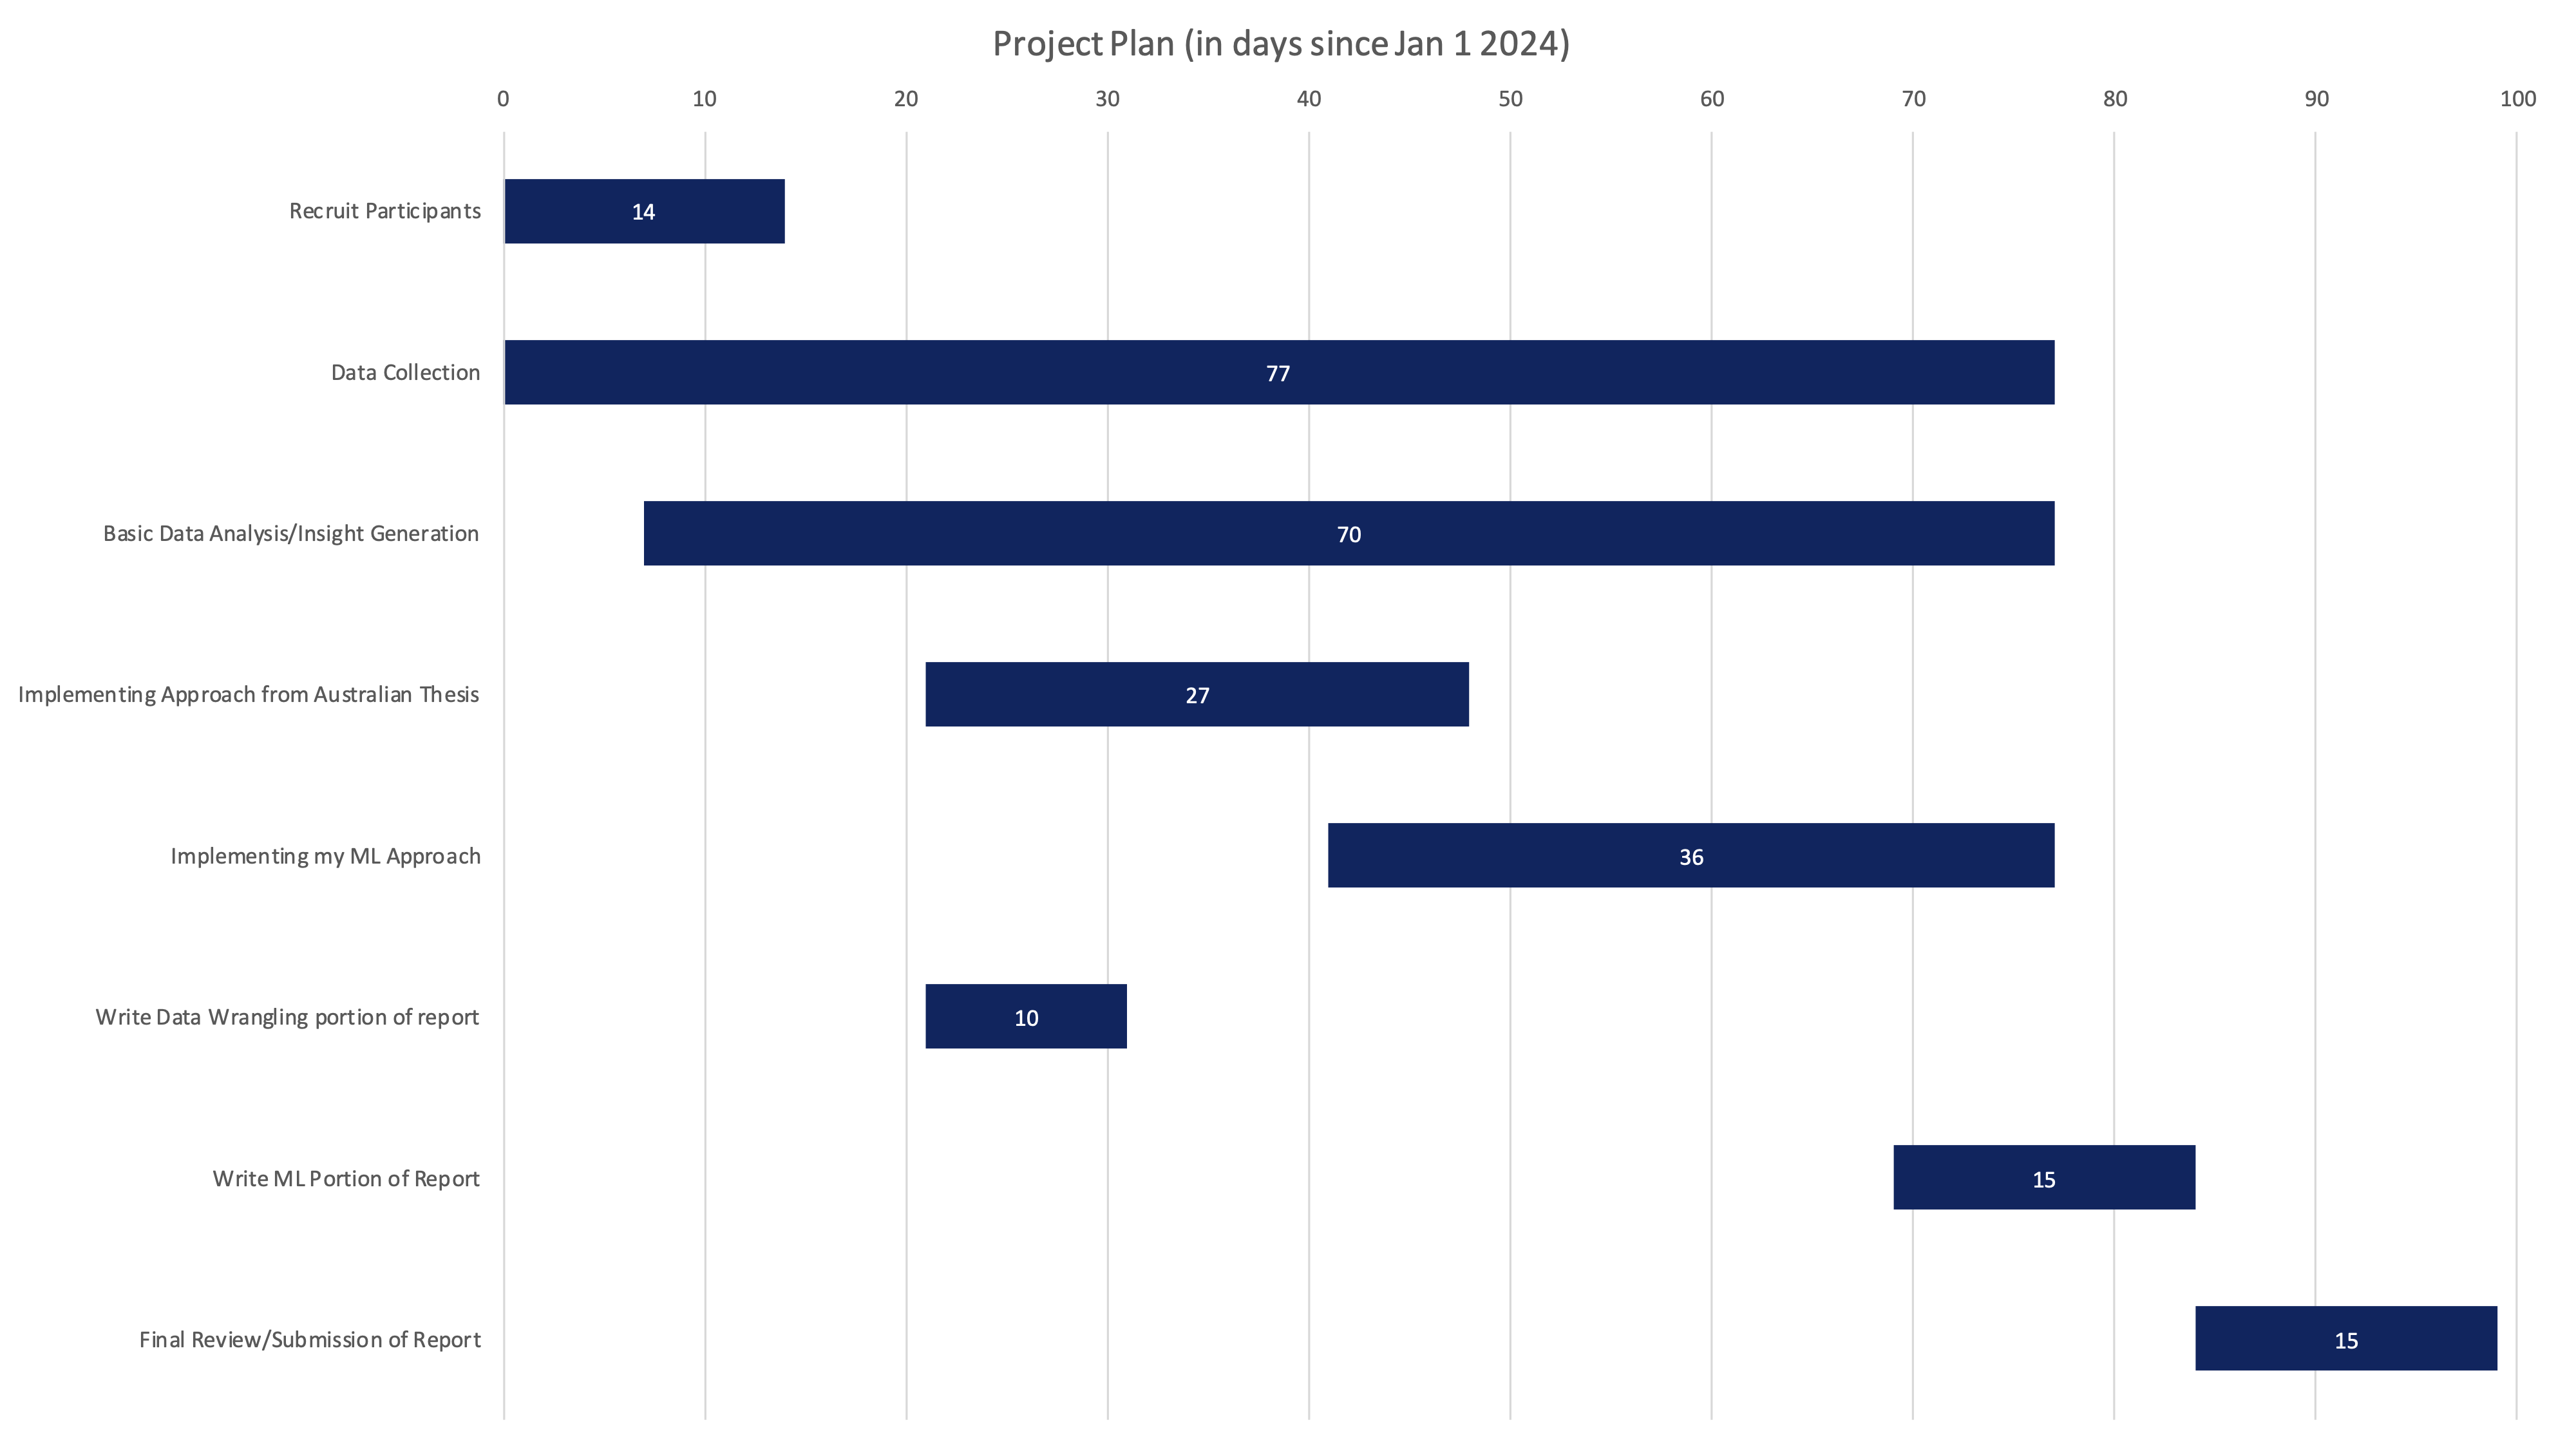
\includegraphics[width=\linewidth]{project_plan.jpg}
\includescalefigure{fig:the_plan}{The Plan}{The Project Plan Gantt Chart}{0.9}{project_plan.png}
}
Data collection and the basic analysis pieces will run throughout most of the project in order to continually provide new data to train models on, as well as to provide feedback to keep participants interested in continuing to provide data to the project. A majority of time is spent actually working on the project with roughly 30 days total dedicated to writing the overall report. Some writing will happen during the course of the development work to make sure I am able to remember what to write about.

\section{The Ethics}
An ethics approval was requested and granted for the collection and storage of user data. There is a wide range of data that could be collected to help provide context to a potential model for training and performance. Data collected includes session data (type, mileage, heart rate, timing) and where available, recovery data (heart rate variability, daily resting heart rate, sleep duration). Stored data will be psuedonomised with a translation key for each participant securely stored on my local machine. Given that the target particpant group would be of a reasonable size, it would take considerable effort for anyone with unauthorised access to figure out which generated key relates to which participant as many training programs are quite similar with similar sessions and timings. Participation for participants is entirely voluntary and they may ask at any time prior to the report due date for their data to be erased from any databases. There is no risk of personal data being revealed as a result of participating in this project. There is a potential for some GPS data to be collected when tracking certain on the water sessions. There is not a risk of personal information being revealed as a result of this GPS data as the locations where on the water rowing takes place are publically known.

% \bibliographystyle{ieeetr}
% \bibliography{refs.bib}
\printbibliography

\end{document}